\section{Results}
\label{sec:results}

All numbers in this section are on the held-out test clips of the synthetic dataset
(Section~\ref{sec:dataset}), unless a real movie is named. Intervals are 95\,\% clip
bootstrap intervals (2000 resamples, the same resamples for every model, so that
differences are paired). Every pass/fail criterion and every prediction quoted here was
fixed before the corresponding number was computed (Section~\ref{sec:protocol}). RQ3 is reported before RQ2 because it
builds on the forecaster of RQ1 directly, while RQ2 adds a separate set of events.

\subsection{Reading the Present}
\label{sec:res-gate1}

Before asking whether forecasts carry physics, we ask whether the frozen encoder carries
it in the present. Each two-frame tubelet is encoded on its own and read by the
attentive and centroid probes of Section~\ref{sec:gate1}.
Table~\ref{tab:gate1} gives the result on the physics stratum.

\begin{table}[h]
  \centering
  \caption{Reading physical observables from one frozen V-JEPA~2 tubelet (test, physics
    stratum). The MSD ceiling is that of a perfect detector at the same frame rate.}
  \label{tab:gate1}
  \begin{tabular}{lcc}
    \toprule
    observable & value & criterion \\
    \midrule
    $R^2$ mean radius & 0.902 & $\geq 0.8$ \checkmark \\
    $R^2$ particle count & 0.726 & $\geq 0.8$ $\times$ \\
    $R^2$ total area & 0.928 & -- \\
    MSD$/4Dt$ & 0.986 (ceiling 0.955) & within 20\,\% \checkmark \\
    \bottomrule
  \end{tabular}
\end{table}

Size, area and diffusion are read at $R^2 \approx 0.9$ and at the perfect-detector MSD,
by an encoder that never saw a microscope image. Count fails the pre-registered bar.
Its error is the same in every crop-edge bucket and largest on reaction and ripening,
the processes with many small particles. This points to shot noise on small particles in
a single frame rather than to merging or to particles cut by the crop edge.
Section~\ref{sec:res-encoder} returns to count when the encoder is adapted.

\subsection{RQ1: Do Forecasts Decode to Physics?}
\label{sec:res-rq1}

\paragraph{Token-level forecasts fade.}
The token-level predictor (Section~\ref{sec:token-forecast}) forecasts all 256 tokens of
the next latent frame. Read through the frozen probes, its forecasts are 76--82\,\%
\emph{worse} than holding the last context frame (persistence) in size-distribution
distance at $+5$, so the pre-registered criterion (Gate~2) fails. The forecasts fade: the
peak occupancy of the predicted particle map falls from 0.96 at $+1$ to 0.69 at $+5$ and
0.44 at $+10$. Readouts trained directly on the forecasts read them about as well as the
last context frame, but find no growth beyond it: the gain in mean-radius error over
persistence is $-0.23$ $[-0.50, +0.03]$\,px on diffusion and $+0.04$ $[-0.21, +0.30]$\,px
on reaction clips.

\paragraph{Why: particles leave their token.}
The failure has a structural cause, which we measured on the simulator's ground truth
(Table~\ref{tab:token-persistence}). Half the particles leave their $16 \times 16$\,px
token within one latent step, and by $+24$ only 6\,\% remain. For a token whose particle
may or may not still be there, the L1-optimal deterministic forecast is background, so
an optimal deterministic token predictor erases particles rather than merely blurring
them, whatever the loss or rollout length. Larger patches keep more of their particles (Figure~\ref{fig:persistence}), but only the whole crop keeps all of them. The same fraction (0.47--0.51 at $+1$) holds
for every process.

\begin{table}[h]
  \centering
  \caption{Token persistence on simulator ground truth (2000 physics-stratum windows,
    $256^2$ crop, 16\,px tokens), measured from the last context frame.}
  \label{tab:token-persistence}
  \begin{tabular}{lccccc}
    \toprule
    horizon (latent steps) & $+1$ & $+2$ & $+5$ & $+10$ & $+24$ \\
    \midrule
    centre still in the same token & 0.49 & 0.37 & 0.23 & 0.15 & 0.06 \\
    old centre still inside the particle & 0.63 & 0.49 & 0.30 & 0.19 & 0.08 \\
    median displacement (px) & 6.9 & 9.7 & 15.3 & 21.3 & 33.1 \\
    \bottomrule
  \end{tabular}
\end{table}

\begin{figure}[t]
  \centering
  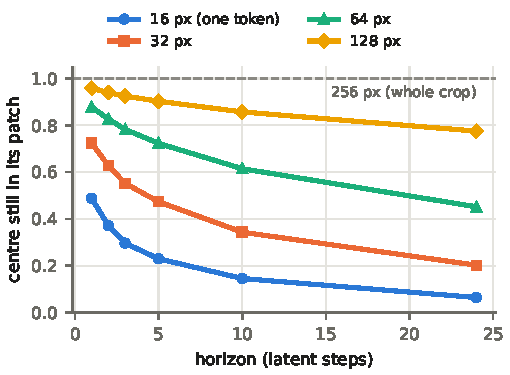
\includegraphics[width=0.55\textwidth]{fig_persistence}
  \caption{Fraction of particles whose centre stays in the same patch, by patch size and horizon, on simulator ground truth. At the token size half leave in one step.}
  \label{fig:persistence}
\end{figure}

What stays predictable is growth. From eight noisy readings of the mean radius, at the
probe's own reading noise, a 20-term ridge regression without labels cuts the $+24$
error from 3.26 / 3.90\,px (persistence) to 1.31 / 1.86\,px on diffusion / reaction
clips. Positions are not predictable; sizes are. This motivates forecasting a
position-free state.

\paragraph{Position-free forecasts carry growth.}
The position-free state is the frame average of the 256 tokens
(Section~\ref{sec:pooled}). A ridge readout from it reads mean radius at $R^2 = 0.877$,
area at 0.942 and count at 0.723, close to the token-level probes, and applied to the
true future latents it recovers growth exponents of 0.311 / 0.473 against the true
$1/3$ / $1/2$. Table~\ref{tab:pooled} compares two label-free forecasters on this state.

\begin{table}[h]
  \centering
  \caption{Position-free forecasting at $+24$ from 8 context frames (test). Gain is the
    reduction in mean-radius error over the pooled trend baseline; exponents are
    median growth exponents read off the forecasts (true: $1/3$, $1/2$, 0).}
  \label{tab:pooled}
  \small\setlength{\tabcolsep}{4pt}
  \begin{tabular}{lccc}
    \toprule
    & \multicolumn{2}{c}{gain over trend (px)} & exponent \\
    \cmidrule(lr){2-3}
    forecaster & diffusion & reaction & diff.\ / react.\ / static \\
    \midrule
    A: linear ridge & $+0.42$ $[+0.15, +0.68]$ & $+0.66$ $[+0.35, +0.98]$
      & 0.208 / 0.269 / 0.008 \\
    B: causal transformer & $+0.54$ $[+0.30, +0.77]$ & $+0.81$ $[+0.59, +1.03]$
      & 0.180 / 0.245 / 0.110 \\
    B $-$ A & $+0.12$ $[-0.18, +0.41]$ & $+0.16$ $[-0.12, +0.43]$ & -- \\
    \bottomrule
  \end{tabular}
\end{table}

Figure~\ref{fig:pooled-forecast} shows the error against horizon. Both forecasters carry each clip's growth beyond the trend, so the size criterion passes
on both processes, but their exponents are damped and miss the $\pm 0.1$ bar (Gate~2$'$
fails for both, as pre-registered). The larger model is not significantly better, and it
invents growth on static clips (0.110).

\begin{figure}[t]
  \centering
  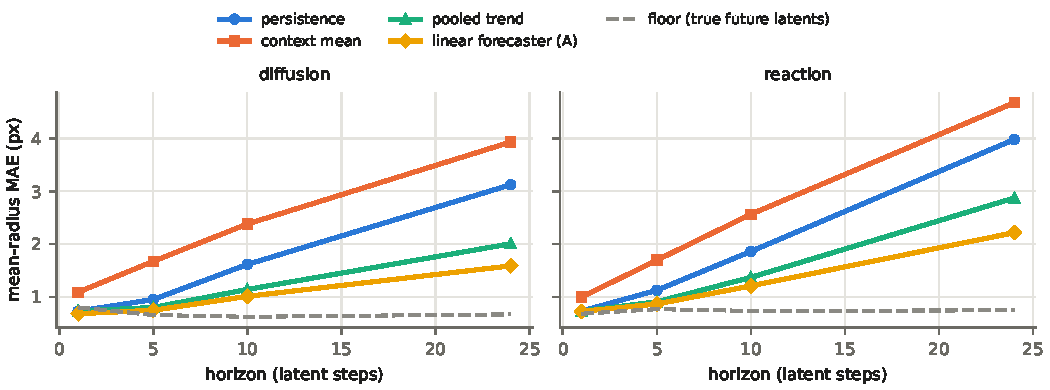
\includegraphics[width=\textwidth]{fig_pooled_forecast}
  \caption{Mean-radius error of the linear position-free forecaster and the trend-blind baselines against horizon (test, physics stratum, context 8). The dashed floor is the readout applied to the true future latents.}
  \label{fig:pooled-forecast}
\end{figure}

\paragraph{The damping is the context's, not the model's.}
Three ground-truth checks locate the exponent shortfall.
\begin{enumerate}
  \item \emph{The bar is out of reach.} With a noise-free context, a nearest-neighbour
    forecaster recovers 0.339 / 0.494. At the probe's reading noise (sd 0.8\,px) the best
    context-only method reaches 0.263 / 0.313. No forecaster can meet the exponent bar
    from eight noisy frames, so that criterion was unpowered.
  \item \emph{A longer context helps by exactly what it allows.} From 8 to 16 context
    frames the linear forecaster's exponents rise by $+0.097$ / $+0.104$ (paired intervals
    above 0) to 0.287 / 0.340, matching the rise of the ceiling itself; the gap to the
    ceiling stays 0.00--0.07. The transformer rises by only $+0.014$ / $+0.027$ and keeps
    inventing growth on static clips: it is limited by the model, the linear map by the
    data.
  \item \emph{A mixture of predictors would not help.} Mode-seeking forecasts undo the
    damping only if the context identifies the process. At the reading noise a router
    picks the right process 33\,\% of the time (chance 20\,\%), and the best single head
    falls to 0.191 / 0.120, below the averaged ridge.
\end{enumerate}

\noindent\textbf{Answer to RQ1: partly.} Deterministic token-level forecasts cannot decode
to correct physics on this instrument. A label-free linear map on the frame-averaged
V-JEPA~2 latent does forecast growth, and its remaining exponent error is what 8--16
noisy frames allow.

\subsection{RQ3: Horizon and Signal-to-Noise Ratio}
\label{sec:res-rq3}

We split the test clips at the median beam flux (21.2; median 12.3 vs 39.3\,e/px in the
two halves) and evaluate the linear forecaster with 16 context frames.

The readout itself is noisier at low dose: its sd-equivalent error is 1.21 vs 0.88\,px,
and it reads particles slightly small (bias $-0.23$\,px). The pre-registered test, low
minus high dose at $+24$, gives $+0.32$ $[-0.20, +1.03]$\,px on diffusion and $+0.28$
$[-0.61, +1.27]$\,px on reaction clips: a penalty is not shown. With about 15 clips per
bin and process this test was close to unpowered, as predicted.

At $+1$ (not pre-registered; Figure~\ref{fig:dose}) the penalty is $+0.41$ / $+0.64$ / $+0.49$\,px on diffusion /
reaction / static clips, all intervals above 0. The penalty stays at 0.3--0.6\,px at every
horizon while the forecast error itself grows, so by $+24$ the error of extrapolating
growth swamps it. For exponents, the ceiling moves by at most 0.034 between dose bins,
against 0.07--0.10 from doubling the context. Over 6--75\,e/px, more frames help growth
recovery more than brighter frames.

\begin{figure}[t]
  \centering
  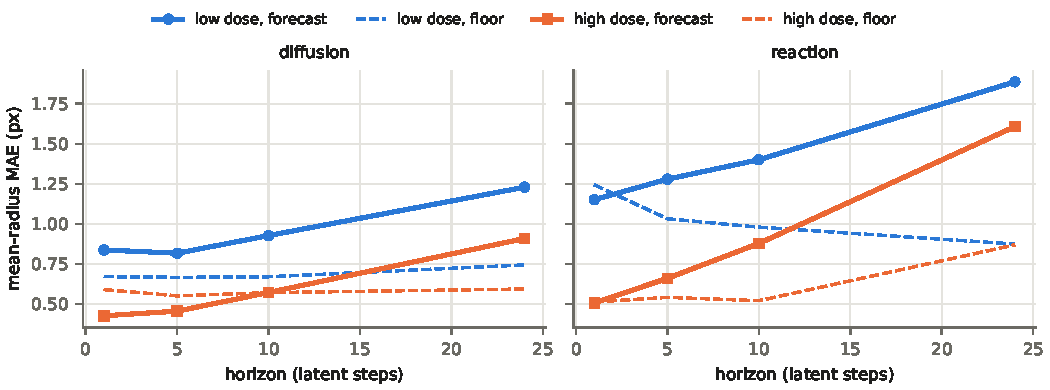
\includegraphics[width=\textwidth]{fig_dose}
  \caption{Error of the linear forecaster (context 16) at low and high electron dose, with the floor of each dose bin (dashed). The low-dose penalty is roughly constant across horizons and enters through the readout.}
  \label{fig:dose}
\end{figure}

\noindent\textbf{Answer to RQ3:} forecast quality degrades strongly with horizon and mildly
with dose, by a roughly constant offset that enters through the readout. The thickness
half of the question is not answered: the mean liquid thickness is fixed at 150\,nm in
the dataset.

\subsection{RQ2: Does Prediction Error Anticipate Coalescence?}
\label{sec:res-rq2}

We take the 48 test-split merges with both particles inside the crop (the 38 validation
merges replicate every reading) and compare signals on the $3 \times 3$-token patch around
each merge against patches around particles far from any merge
(Table~\ref{tab:merges}).

\begin{table}[h]
  \centering
  \caption{Separating merge patches from non-merge particle patches (AUC, test).}
  \label{tab:merges}
  \begin{tabular}{lcc}
    \toprule
    signal & at the merge & one step before \\
    \midrule
    token forecaster's $+1$ error & \textbf{0.710} $[0.618, 0.793]$ & 0.592 \\
    raw latent change & 0.635 & 0.550 \\
    distance from the context average & 0.738 & 0.661 \\
    token brightness change (pixels) & 0.704 & 0.657 \\
    frame-averaged forecaster's $+1$ error & 0.598 $[0.524, 0.679]$ & 0.569 \\
    \bottomrule
  \end{tabular}
\end{table}

The forecaster's error is larger where two particles merge than where one just moves,
so it \emph{detects} merges (Figure~\ref{fig:merges}). It is not a specific detector: it beats only the raw latent
change ($+0.075$ $[+0.033, +0.112]$, by denoising it) and ties the context average and the
pixel signal. It does not \emph{anticipate} merges: one step before contact every signal
is above chance, pixels included, because a pre-merge patch already holds two particles,
and the forecaster adds nothing to that ($-0.065$ against pixels). One step after the
merge its AUC falls to 0.57 while the context average and the pixels stay near 0.70: the
forecaster has seen the merged particle and now forecasts it. To a deterministic
forecaster, a random encounter is a one-frame surprise. The position-free forecaster's
error, computed on the whole frame, separates merges less well (0.598): averaging over the
frame dilutes a change that happens in one place.

\begin{figure}[t]
  \centering
  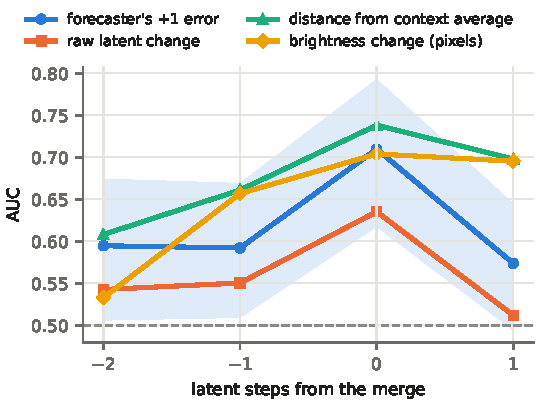
\includegraphics[width=0.6\textwidth]{fig_merges}
  \caption{Separating merge patches from patches around moving particles, by latent steps from the merge (test, 48 merges). The band is the 95\,\% interval of the forecaster's error. No signal anticipates the merge beyond the cue that two particles are already close, and the forecaster adapts one step after it.}
  \label{fig:merges}
\end{figure}

\noindent\textbf{Answer to RQ2:} prediction error detects coalescence as it happens but does
not anticipate it, and simple baselines detect it equally well.

\subsection{Transfer to Real LPTEM Video}
\label{sec:res-real}

Published supplementary movies are not usable as data without screening
(Section~\ref{sec:real-data}): of 132 movies from 34 papers, 10 keep detector pixels and
time steps intact; we use 8 from 7 papers, plus the Au nanorod video of SAM-EM.
Table~\ref{tab:real} gives four checks, from the input to the forecast.

\begin{table}[h]
  \centering
  \caption{Real movies against simulation. A: nearest-neighbour containment of the
    pooled latents (limit 1.50, the largest held-out synthetic clip). B: readout over
    pixel estimate of mean radius. C: sign of growth, readout vs pixels. D: forecaster
    gain over the context mean at $+24$.}
  \label{tab:real}
  \begin{tabular}{ll>{\raggedright\arraybackslash}p{7.2cm}}
    \toprule
    check & simulation & real \\
    \midrule
    A & median 0.93 & nanorods 1.51; six other bright-field movies 3.2--8.6;
      HAADF control 2.58 \\
    B & median 1.11 (band 0.79--1.74) & 0.46--1.00; 2 of 5 movies in the band \\
    C & -- & disagree on one movie ($\rho = -0.87$ vs $+0.79$, 35 blocks) \\
    D & $+0.061$ $[+0.045, +0.078]$ & $-0.418$ $[-0.511, -0.286]$; negative on every
      movie, already at $+1$ \\
    \bottomrule
  \end{tabular}
\end{table}

No real movie lies inside the simulated feature distribution (Figure~\ref{fig:containment}). The movie the simulator was
calibrated on comes nearest and sits at the limit (1.51 against 1.50); every other one is
far outside. The readout reads real particles small, and the forecaster loses to the
context mean on every movie from the first step. It fails at the input, not through
extrapolation: real pooled latents change less per step than simulated ones (one-step
error of the context mean 0.30 vs 0.40), yet the forecaster's one-step error doubles
(0.65 vs 0.40). Of the four predictions made for these checks, A was wrong (bright-field
movies were expected inside), B mostly wrong, C mixed and D right. The claims of this
thesis are therefore scoped to simulation.

\begin{figure}[t]
  \centering
  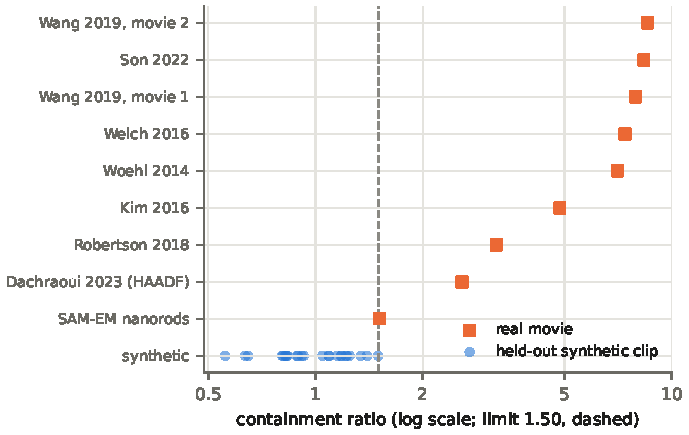
\includegraphics[width=0.7\textwidth]{fig_containment}
  \caption{Containment of each real movie's pooled latents against the simulated ones (check A): the ratio of the distance to the nearest synthetic sample over the typical synthetic-to-synthetic distance. The dashed line is the largest ratio of a held-out synthetic clip.}
  \label{fig:containment}
\end{figure}

\subsection{Frozen, Adapted or From Scratch: The Encoder}
\label{sec:res-encoder}

Section~\ref{sec:res-gate1} used the encoder frozen. To see what that choice costs, we
compare it with the same encoder adapted by LoRA (\textsf{L}, 7.62\,M trainable
parameters) and with a small CNN trained from scratch (\textsf{C}, 1.51\,M parameters),
with everything but the encoder held fixed (Section~\ref{sec:method-encoder}). Table~\ref{tab:encoders} and Figure~\ref{fig:data-efficiency} give the result.

\begin{table}[h]
  \centering
  \caption{Encoder comparison (test, physics stratum). Reading sd is the mean-radius
    error in sd-equivalent pixels.}
  \label{tab:encoders}
  \begin{tabular}{llcccc}
    \toprule
    data & enc. & $R^2$ count & $R^2$ mean radius & $R^2$ area & reading sd (px) \\
    \midrule
    100\,\% & \textsf{F} & 0.726 & 0.902 & 0.928 & 0.93 \\
            & \textsf{C} & 0.838 & 0.950 & \textbf{0.978} & 0.63 \\
            & \textsf{L} & \textbf{0.843} & \textbf{0.951} & 0.976 & \textbf{0.62} \\
    \midrule
    30\,\%  & \textsf{F} & 0.646 & 0.872 & 0.910 & 1.06 \\
            & \textsf{C} & 0.757 & 0.918 & 0.943 & 0.89 \\
            & \textsf{L} & \textbf{0.781} & \textbf{0.941} & \textbf{0.946} & \textbf{0.69} \\
    \midrule
    10\,\%  & \textsf{F} & 0.587 & 0.819 & 0.859 & 1.25 \\
            & \textsf{C} & 0.661 & 0.864 & 0.910 & 1.09 \\
            & \textsf{L} & \textbf{0.726} & \textbf{0.922} & \textbf{0.931} & \textbf{0.83} \\
    \bottomrule
  \end{tabular}
\end{table}

The frozen encoder is the weakest at every data size, on every $R^2$, on reading sd and on
detection F1 (0.83 against 0.87--0.89). A small CNN trained from scratch beats it by
0.07--0.11 on count. The frozen features carry the information (LoRA starts from exactly
them), but not in a form the probes read well. Adapting the encoder is what pays, and it
pays most when labels are few: at 100\,\% LoRA and the CNN tie (every difference within
$\pm 0.005$, intervals spanning 0), while at 10\,\% LoRA leads the CNN by 0.065 on count
and 0.06 on mean radius, and LoRA on 160 clips matches the frozen encoder on 1600. We had
predicted that pretraining would pay with few labels even without adaptation; it does
not ($F - C = -0.075$ $[-0.121, -0.031]$ on count at 10\,\%).

\begin{figure}[t]
  \centering
  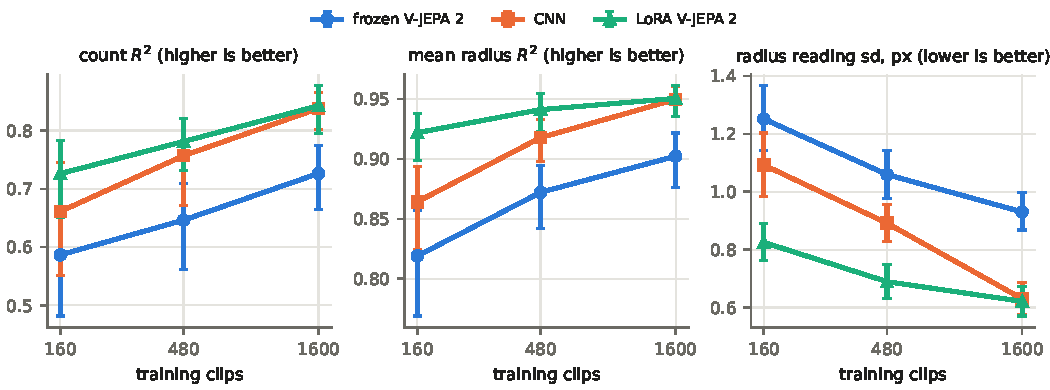
\includegraphics[width=\textwidth]{fig_data_efficiency}
  \caption{Encoder comparison against the number of training clips (test, physics stratum, 95\,\% intervals). LoRA on 160 clips matches the frozen encoder on 1600.}
  \label{fig:data-efficiency}
\end{figure}

Positions were never the bottleneck: MSD$/4Dt$ is within 6\,\% of the perfect-detector
ceiling for every encoder. Low dose costs every encoder about 0.2\,px of reading sd;
better encoders lower both dose bins rather than closing the gap, so the penalty is a
property of the frames.

Does the better reading change RQ1? We had fixed in advance that the position-free
forecaster would be rerun on the adapted encoder if its reading sd fell to 0.6\,px or
below. LoRA reads 0.621 $[0.571, 0.674]$\,px, so the rerun is not triggered, and the
exponent analysis of Section~\ref{sec:res-rq1} stands with the frozen encoder. The margin
is well inside the noise.

\subsection{Summary}
\label{sec:res-summary}

Table~\ref{tab:summary} collects the answers. Read together, the results separate what a
frozen video model can and cannot do on this instrument. It reads the present well, size
and diffusion close to their ceilings, and an adapted encoder reads it better still. What
it cannot do is forecast where particles go: the motion is random at the scale of a token,
so a deterministic forecast of the tokens erases the particles, and its prediction error
marks merges only once they have happened. What it can forecast is the position-free part
of the state, the growth of the particle population, up to the limit set by how noisy and
how short the context is; and how much that limit costs depends more on the number of
context frames than on the electron dose. All of it holds in simulation and none of it on
the real movies we could obtain.

\begin{table}[H]
  \centering
  \caption{Answers to the research questions.}
  \label{tab:summary}
  \begin{tabular}{>{\raggedright\arraybackslash}p{4.2cm}>{\raggedright\arraybackslash}p{9.8cm}}
    \toprule
    question & answer \\
    \midrule
    RQ1: do predicted latents decode to correct future physics?
      & Partly. Token-level forecasts erase particles for a structural reason. A
        label-free linear forecaster on the frame-averaged latent carries growth; its
        exponents are damped by the information limit of the noisy context. \\ \addlinespace
    RQ2: does prediction error anticipate coalescence?
      & It detects merges (AUC 0.71) but does not anticipate them, and simple baselines
        detect them as well. \\ \addlinespace
    RQ3: how does quality degrade with horizon and SNR?
      & Strongly with horizon, mildly with dose (0.3--0.6\,px at every horizon, through
        the readout). Context length matters more than dose for exponents. \\ \addlinespace
    Real data
      & No transfer: real movies lie outside the simulated feature distribution, and the
        forecaster loses to the context mean on every movie. \\ \addlinespace
    Encoder
      & Frozen V-JEPA~2 is the weakest reader; LoRA adaptation ties a CNN with full data
        and leads it with 10\,\% of the labels. \\
    \bottomrule
  \end{tabular}
\end{table}
